\documentclass[sigconf]{acmart}
\usepackage[flushleft]{threeparttable}
\usepackage[shortlabels]{enumitem}
\usepackage{subfigure}

\AtBeginDocument{%
  \providecommand\BibTeX{{%
    \normalfont B\kern-0.5em{\scshape i\kern-1000.25em b}\kern-0.8em\TeX}}}

\setcopyright{acmcopyright}
\copyrightyear{2018}
\acmYear{2022}
\acmDOI{10.1145/1122445.1122456}

\acmConference[CIKM '22]{CIKM '22: 31st ACM International Conference on Information and Knowledge Management}{Oct 17--22, 2022}{Atlanta, Georgia, USA}
\acmBooktitle{CIKM '22: 31st ACM International Conference on Information and Knowledge Management}
\acmPrice{15.00}
\acmISBN{978-1-4503-XXXX-X/18/06}

\begin{document}

\title{Building a Best Buy Store Interactive Webpage Using Django}

\author{Morgan Brockman}
\affiliation{%
    \institution{University of Idaho}
        \streetaddress{875 Perimeter Drive}
        \city{Moscow}
        \state{Idaho}
        \country{USA}
        \postcode{83843}
}
\email{broc7795@vandals.uidaho.edu}

\author{Ian Fleming}
\affiliation{%
    \institution{University of Idaho}
        \streetaddress{875 Perimeter Drive}
        \city{Moscow}
        \state{Idaho}
        \country{USA}
        \postcode{83843}
}
\email{flem8015@vandals.uidaho.edu}


\begin{abstract}

We set out to apply Database Structure concepts in the practical setting of building an interactive website. To do this, we used Django, the popular python-based web framework. This involved using the SQLite3 database, Django's default included database, and a good option for portability, though most database interaction was done through Django-provided functions. While Django simplified the process of interaction with the database directly, freeing up focus for website polish and features, a majority of our time was spent learning to work with Django and its functionality.

\end{abstract}

%%
%% The code below is generated by the tool at http://dl.acm.org/ccs.cfm.
%% Please copy and paste the code instead of the example below.
%%
\begin{CCSXML}
<ccs2012>
   <concept>
       <concept_id>10003033.10003099.10003037</concept_id>
       <concept_desc>Networks~Naming and addressing</concept_desc>
       <concept_significance>300</concept_significance>
       </concept>
   <concept>
       <concept_id>10003033.10003099.10003104</concept_id>
       <concept_desc>Networks~Network management</concept_desc>
       <concept_significance>300</concept_significance>
       </concept>
   <concept>
       <concept_id>10011007.10011006.10011008.10011009.10011011</concept_id>
       <concept_desc>Software and its engineering~Object oriented languages</concept_desc>
       <concept_significance>300</concept_significance>
       </concept>
   <concept>
       <concept_id>10011007.10011006.10011008.10011009.10011019</concept_id>
       <concept_desc>Software and its engineering~Extensible languages</concept_desc>
       <concept_significance>500</concept_significance>
       </concept>
   <concept>
       <concept_id>10011007.10011006.10011008.10011024.10011029</concept_id>
       <concept_desc>Software and its engineering~Classes and objects</concept_desc>
       <concept_significance>300</concept_significance>
       </concept>
   <concept>
       <concept_id>10011007.10011006.10011008.10011024.10011026</concept_id>
       <concept_desc>Software and its engineering~Inheritance</concept_desc>
       <concept_significance>300</concept_significance>
       </concept>
   <concept>
       <concept_id>10011007.10011006.10011008.10011024.10011031</concept_id>
       <concept_desc>Software and its engineering~Modules / packages</concept_desc>
       <concept_significance>500</concept_significance>
       </concept>
   <concept>
       <concept_id>10011007.10011006.10011008.10011024.10011033</concept_id>
       <concept_desc>Software and its engineering~Recursion</concept_desc>
       <concept_significance>300</concept_significance>
       </concept>
   <concept>
       <concept_id>10011007.10011006.10011066.10011070</concept_id>
       <concept_desc>Software and its engineering~Application specific development environments</concept_desc>
       <concept_significance>500</concept_significance>
       </concept>
   <concept>
       <concept_id>10011007.10011006.10011066.10011067</concept_id>
       <concept_desc>Software and its engineering~Object oriented frameworks</concept_desc>
       <concept_significance>300</concept_significance>
       </concept>
   <concept>
       <concept_id>10002951.10002952.10002953.10002955</concept_id>
       <concept_desc>Information systems~Relational database model</concept_desc>
       <concept_significance>500</concept_significance>
       </concept>
   <concept>
       <concept_id>10002951.10002952.10002971.10003450</concept_id>
       <concept_desc>Information systems~Data access methods</concept_desc>
       <concept_significance>300</concept_significance>
       </concept>
   <concept>
       <concept_id>10002951.10002952.10003190.10003205</concept_id>
       <concept_desc>Information systems~Database views</concept_desc>
       <concept_significance>500</concept_significance>
       </concept>
   <concept>
       <concept_id>10002951.10002952.10003190.10003206</concept_id>
       <concept_desc>Information systems~Integrity checking</concept_desc>
       <concept_significance>100</concept_significance>
       </concept>
   <concept>
       <concept_id>10002951.10003260.10003282.10003550.10003552</concept_id>
       <concept_desc>Information systems~E-commerce infrastructure</concept_desc>
       <concept_significance>300</concept_significance>
       </concept>
 </ccs2012>
\end{CCSXML}

\ccsdesc[300]{Networks~Naming and addressing}
\ccsdesc[300]{Networks~Network management}
\ccsdesc[300]{Software and its engineering~Object oriented languages}
\ccsdesc[500]{Software and its engineering~Extensible languages}
\ccsdesc[300]{Software and its engineering~Classes and objects}
\ccsdesc[300]{Software and its engineering~Inheritance}
\ccsdesc[500]{Software and its engineering~Modules / packages}
\ccsdesc[300]{Software and its engineering~Recursion}
\ccsdesc[500]{Software and its engineering~Application specific development environments}
\ccsdesc[300]{Software and its engineering~Object oriented frameworks}
\ccsdesc[500]{Information systems~Relational database model}
\ccsdesc[300]{Information systems~Data access methods}
\ccsdesc[500]{Information systems~Database views}
\ccsdesc[100]{Information systems~Integrity checking}
\ccsdesc[300]{Information systems~E-commerce infrastructure}

\ccsdesc[500]{Information systems~Resource Description Framework (RDF)}
\ccsdesc[500]{Computing methodologies~Natural language processing}
\ccsdesc[500]{Computing methodologies~Knowledge representation and reasoning}
\ccsdesc[500]{Information systems~Question answering}
\ccsdesc[300]{Information systems~Graph-based database models}
\ccsdesc[300]{Information systems~Web Ontology Language (OWL)}

\keywords{Web Development, Web Framework, Django, Python, SQLite3, HTML5, CSS, Visual Studio Code, GitHub, Database Systems, Discord}

\maketitle

\pagebreak
\section{Development Tools}
Many different development tools were utilized in the development of this web page. Each development tool listed here contributed massively to the development's workflow and our productivity in the project development. Missing any one of these tools would have massively altered the development process for this website.

\subsection{VSCode}
We both made heavy use of VSCode, a popular, fully featured, heavily-extensible text editor designed for a wide range of programming situations. The most obvious feature utilized was VSCode's syntax highlighting and auto-completion. The program scrapes your project's files, imported packages, and relevant classes, and provides context-aware auto completion suggests, or highlights relevant variables. The program also features many productivity-increasing text-editing features, such as split view windows, auto and bulk indentation, multi-line editing, and much more. Another huge source of functionality is VSCode's extensibility. Through first party and community extensions, nearly endless functionality can be added to VSCode's application, such as in-app git control, LaTeX editing, viewing, and building, and more to be covered in the following subsections.

\subsection{git Version Control}
The version control software git allows developers to track changes made to their software verbosely, robustly, and indefinitely. Every time me made a change or added a feature to our app, we recorded the changes as well as a message describing the change using git. In doing so, git allowed us to keep close track of the progress of our development, and exactly what changes where made when. It also allowed very simple reversion to previous changes, when the situation arose.

\subsection{GitHub Collaboration Service}
Not entirely separate from git, but a service all on it's own, is Github. GitHub's git repository functionality allowed us to combine Git's version control features with a remote repository, allowing us to develop the project on two separate machines, at two separate locations. Whenever a change is tracked with git, it must be stored in the Github repository to truly be tracked. Once this is done, the repository acts as an intermediary between us, managing our changes to the code and the times they were made, keeping track in order to merge our changes and share them between us. 

\pagebreak
\subsection{Discord Communication Service}
Almost all of our communication was done over the Discord communication app. Having an easily accessible go-to method for communication is a necessity for any collaborative work. Discord's ability to communicate via text, speak over voice calls, share files, and even share real-time code manipulation was all essential to our collaborative development.

\subsection{VSCode Database Viewer}
As mentioned previously, VSCode offers a plethora of extensions to enhance its feature-set. One such extension is any of several database viewer extensions. These extensions allowed easy, simple, real-time viewing of our application's database, as well as the database's structure and data types of every field.

\subsection{dbdiagram.io Database Diagram Builder}
This website allows designing of relational database models through clear and easy to follow pseudo-code. By simply following the provided example code and changing the values, the site automatically generates an intractable image representation of your database. The website also allows exporting of the generated image with little to no extra hassle, only requiring a watermark on the final image, as can be seen later in this paper.

\subsection{Django Development Server}
In the use of the Django Web Framework, our app and website can be locally hosted from our own machines. This enables us live feedback for any changes we make on multiple axes. This is only possible if we first host a Django virtual environment. The purpose of a virtual environment is quite tactful as it prevents permanent errors from blooming and the ability to manipulate the state machine in anyway without affecting one's machine or static environment. In addition, a benefit of this is the detailed error pages generated by Django for the back-end and its error-handling.

\section{Development Languages}
The following are technical descriptions of the programming languages this project was built off of.

\subsection{Python}
The Django Web Framework utilizes the Python language for all of its back-end development and implementation. We used Python version 3.8.10. Python proved to be straightforward to learn and to utilize as the syntax is very light and the libraries are easy to use. The only downside in using Python is its performance, but our project didn't seem to experience such issues.

\pagebreak
\subsection{SQL}
Our project utilized the SQLite3 framework for the data base implementation. This framework proved the most effective and reliable for our project for it is lightweight and functions quite well in Python and Unix environments.

\subsection{HTML}
HTML5 was utilized for the front-end development of our project. As a styling/design language, it was relatively straightforward to learn and program. Our project utilizes multiple pages in HTML that create the overall structure as it may appear on the Internet. Furthermore, the use of HTML enabled the possibility of back-end functionality such as user input and feedback.

\subsection{CSS}
The latest version of CSS is responsible for graphical styling and the creation of visual hierarchy amongst all of our web pages in our project. We have a primary style sheet that essentially resets the styling for the main elements prior to anything. This is a good coding practice. The rest of the pages utilize their own style sheet for organization sake and the prevention of conflict. All of our styling in CSS was coded from the ground-up and was pure.


\section{Development}\label{development}
The development process was very simply structured into three rather distinct parts. First, there was the design of the database that would be running under the hood of our website. Then, there was the development of the website, which would be separated pretty cleanly between the back-end development, working with Django's various functions and features, and the front-end development, working with the HTML, CSS, and Django's templating features. We both worked together on the design of the database. Morgan primarily focused with Django's functions, while Ian worked with Django's HTML templating system and the website's front-end.

\subsection{Database Design}\label{database}
% talk about actual design process
Our database design was relatively simple with how many tutorials there were online for similar websites. We followed Mozilla's tutorial for building a website for a library using Django, and it's database design mapped pretty well to ours. \par
All products are contained in the Product table. Each product has its own unique UUID, a 36 character uniquely-generated identifying string, with a special datatype built into Django. This serves as the table's primary key. \par
Within the Product table are several one-to-one foreign key relationships for the various features available. These are each stored in tables which simply contain an iterating id primary key and the name for the relevant feature. Doing this allowed us to make querying matching products very simple. \par
\pagebreak
Aside from this there are several less important fields which are simply stored as their own relevant variables within the table itself. This allowed for more flexibility in storage, though it did make querying them a bit more involved. \par
We then used Mockaroo to generate data matching the tables and populate our database.

\begin{figure} [H] % [H] forces the figure to be placed exactly where it appears in the text
	\centering % Horizontally center the figure
	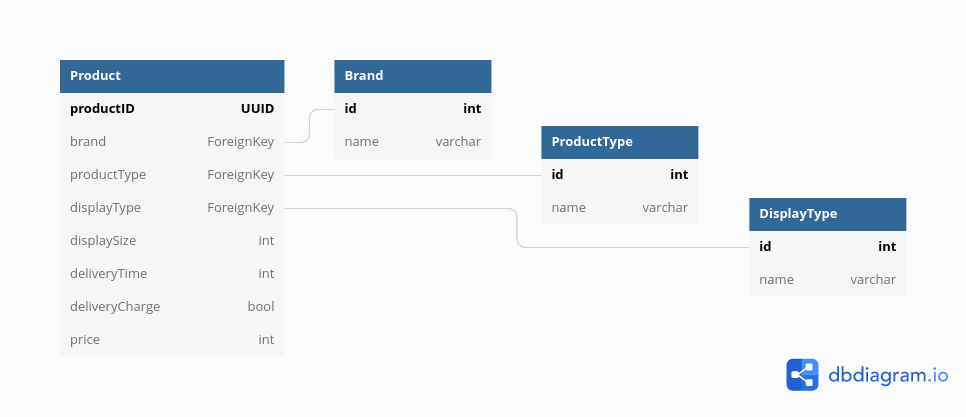
\includegraphics[width=0.48\textwidth]{Figures/databaseRelations} % Include the figure
	\caption{Relational database diagram for Best Buy website}
\end{figure}

\subsection{Django}\label{django}
%Talk about how learning django went
Much of our time spent on the project was learning how to work with Django's vast and extensible feature-set. For brevity, a simplified description of how building a website with Django works can break it down into the following three feature.

\hspace{1em}\begin{description}
	\item[models.py] \hfill \\
	Rather than working with any particular database system directly, Django abstracts this work with its models feature. Using conventions defined by Django, the developer can design their database using more abstract database design concepts more directly. Tables are defined as classes, with variables belonging to that class being treated as forms within that table. These variables are extremely extensible through Django's documentation, allowing the developer to do this such as: defining the primary key, linking another table as a foreign key, defining the forms data types (such as integers, bools, dates, or times), or even automatically generating standardized UUIDs (universally unique identifiers) salted through your MAC address, namespace hashes, or a plethora of other methods at the developer's choosing. \par
	Once these models are implemented, Django handles building and modifying them on its own, regardless of the database one chooses. Switching databases is as simple as modifying a settings file and possibly installing the Django package for its support. Often, depending on the previous database implementation, data migration between databases is as simple as a Django command.
\pagebreak
	\item[views.py] \hfill \\
	Paired with Django's models feature is the views feature. This allows the developer to define variables and functions, take GET and POST calls, manipulate both and pass the results to the generated HTML page. Along with all the functionality for creating dynamic web pages this allows by simply effectively extending HTML with Python and everything that offers, a particularly important feature is Django's object.filter() function. This effectively abstracts SQL queries from the previously defined models to more python friendly if statements and equality operators. \par
	The process for dynamic web page deployment in essence becomes: deliver a web pages data with python, return any data through HTML POST, retrieve that data from models using python, and deliver the new web page with python.
	\item[HTML Templates] \hfill \\
	The HTML templates provided by Django were organized in such a fashion where the user is given a basic/generic
	page responsible for the general HTML/head data and styles that the web pages will be governed by. Any other web pages (including the index.html) created by the user will inherit or extend from this basic/generic page. Embedded commands provided from Django are used in each web page to produce content based on the back-end functionality.
\end{description}

\subsection{Website Design}\label{website}
Our project aimed to delivery visual simplicity alongside effective functionality. Our website was designed to be easily navigable and interactive. Our color schema mimicked that of Best Buy's alongside other contrasting elements. We used the Open Sans font family because it is visually pleasing and concise with its various font weights. We aimed to have elements on all pages to be equally spaced and centered for a professional and forward appeal. Furthermore, we added simple animations to certain elements (i.e. buttons) to add flair and personality. The front-end styling behind our website is pure CSS and not assisted with Bootstrap or any other applet alike. In short, we wanted to craft a website that was personable and simplistic while delivering the services our users want effectively.

\subsection{Deployment and Hosting}\label{hosting}
%move
Django bundles with it its own entirely self-contained development server. While this is primarily intended for development on a local machine, and while the practice does not necessarily follow best security practices, the development server is entirely extensible through only a few settings changes. For out particular project, we are simply using a domain Morgan happened to already own. Using Google Site's interactive settings, we simply pointed the desired subdomain to a specific port, forwarded that port on the development machine's local network, and the website is now fully accessible whenever the development server is running.

\pagebreak
\subsection{HTML Templates}\label{templates}
In our use of the Django web framework, we utilized the provided basic/generic web page. Here, we included all of our style sheets and other various "head" data and information. A stylistic and functional navigation bar was added to this page so that it would be present for all other pages that extend from it. Here on, we created the rest of the necessary pages our project would need and had them extend from our basic/generic. Each had their own style sheet loaded statically from the page as well. This structure worked most effectively and allowed the front-end development much more seamless and organized.

\section{Database}
We used SQLite3 to implement the website's database, as it works well with Django out of the box, and its portable nature made collaboration using git much easier than many alternatives. \par
Our database is made of of four tables: a larger product table, and three short feature tables. \par
Pictures provided are from the website's admin interface, where table data can be graphically viewed or modified.

\subsection{Brands}
Our Brand table contains only an automatically iterating ID integer as its primary key and a variable character field as its name.\par
For each brand or make of product available, an entry is stored in this table, and then referenced by a one-to-one foreign key in the product table. This allows easy listing and searching of all the available product brands.

\begin{figure}[H] % [H] forces the figure to be placed exactly where it appears in the text
    \centering
	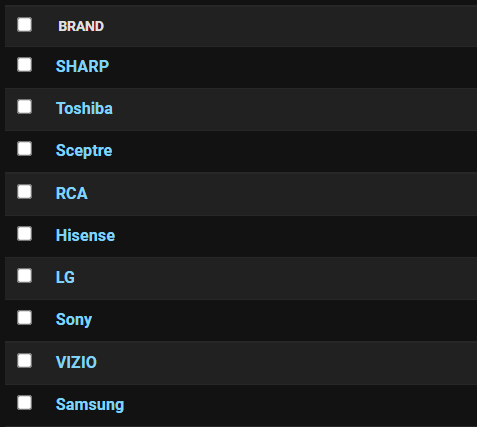
\includegraphics[width=0.48\textwidth]{Figures/brands.png} % Include the figure
	\caption{Picture of the Brands table.}
\end{figure}

\pagebreak
\subsection{Product Types}
Like the Brand table, the Product Types table contains only an automatic iterating ID integer as its primary key and a variable character field as its name. \par
This table contains an entry for every type of product available in the store. Like the brands, the product table may contain a one-to-one foreign key referencing a particular type of product in this table.

\begin{figure}[H] % [H] forces the figure to be placed exactly where it appears in the text
	\centering % Horizontally center the figure
	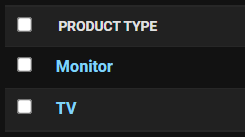
\includegraphics[width=0.4\textwidth]{Figures/producttype.png} % Include the figure
	\caption{Picture of the Product Type table.}
\end{figure}

\subsection{Display Types}
Like the previous two tables, the Display Types table contains only an automatic iterating ID integer as its primary key and a variable character field as its name. \par
Each entry in this table represents a different type of display technology available in the store. Like the other two feature tables, the product table may contain a one-to-one foreign key referencing a single type of display technology listed in this table.

\begin{figure}[H] % [H] forces the figure to be placed exactly where it appears in the text
	\centering % Horizontally center the figure
	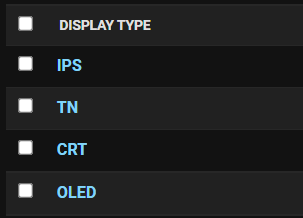
\includegraphics[width=0.45\textwidth]{Figures/displaytypes.png} % Include the figure
	\caption{Picture of the Display Type table.}
\end{figure}

\pagebreak
\subsection{Products}
Our products table is where the bulk of the information is stored. For each product available in the website, there is an entry on this table. \par
Each entry contains a unique UUID (Universally Unique Identifier) acting is the entry's primary key. The UUID is a special 36bit Django data field, automatically generated at instantiation whenever a product is added to the table. \par
Each entry also contains three foreign keys, one for each feature which is common to many products: Brand, Product Type, and Display Type. The available data for each of these features is stored in separate feature tables, as described previously. The foreign keys each mark one-to-one relationships with a single product in each of their feature tables. \par
The other fields of the product table contain more specific information on a given product. The displaySize field denotes in inches the size of the product's display, if it has one. This is simply stored as an integer. The deliveryTime field denotes in days how long the product's delivery time is estimated to take. This is also a simple integer field. The deliveryCharge field is a boolean denoting whether or not a given product charges paid delivery. The price field self-evidently stores the product's price. This is again a simple integer field denoting the price in USD.


\begin{figure}[H] % [H] forces the figure to be placed exactly where it appears in the text
	\centering % Horizontally center the figure
	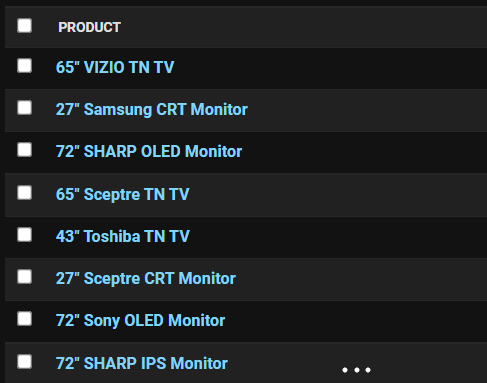
\includegraphics[width=0.48\textwidth]{Figures/product.png} % Include the figure
	\caption{Picture of the Product table.}
\end{figure}

\subsection{Mockaroo}

Mockaroo is a website service that provides the user the ability to create mock data in various formats for a database. Our project utilizes and is dependent on mock data for the functionality of the database as a whole. We had it so multiple columns would be present to function as characteristics or features of a product and the values of each would vary and generate randomly.

\pagebreak
\section{Functionality}\label{functionality}
%walk through using each page like a baby. then talk about how the html is laid out, followed by how view is laid out
The following sections will describe the front-end implementations and the back-end implementations of each page.

\subsection{Home Page}\label{home}

Functionally, the front-end development of the home page is quite simple and straight-forward. A basic splash/welcome page is produced alongside three buttons. These three buttons, labeled: "by UUID", "by Feature", and "by Requirement" are responsible for redirecting the user to the page of the particular searching criterion they desire. \par
These buttons feature Django HTML Template function calls which automatically handle URL Mapping to the correct view function, taking the user to the given URL and generating for them a dynamic HTML page, depending on the selected search feature. 

\begin{figure}[H] % [H] forces the figure to be placed exactly where it appears in the text
	\centering % Horizontally center the figure
	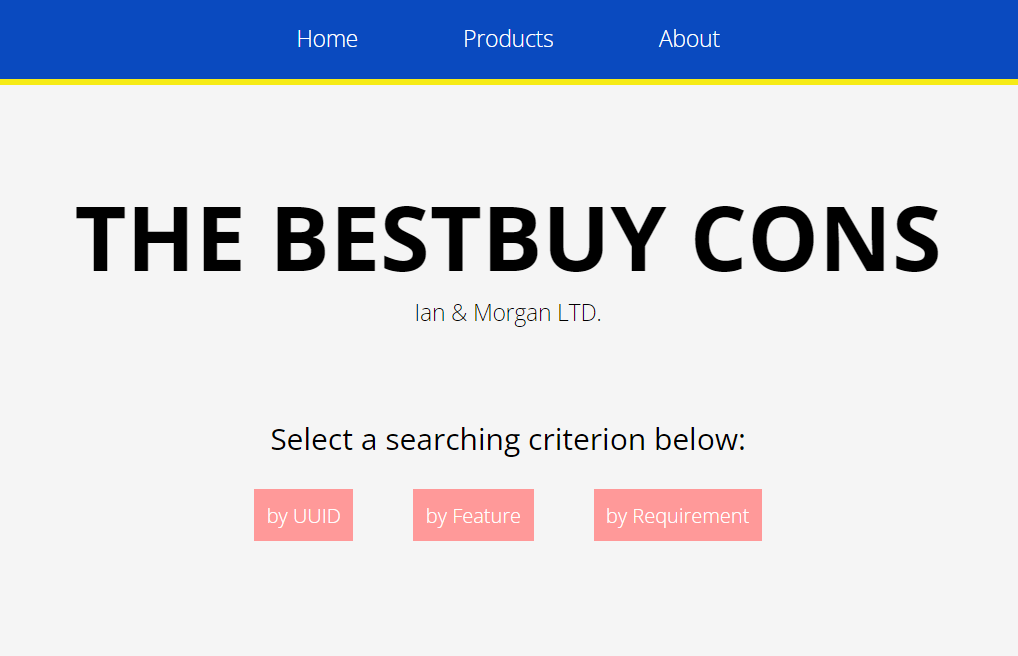
\includegraphics[width=0.48\textwidth]{Figures/index.png} % Include the figure
	\caption{Picture of the home page.}
\end{figure}

\subsection{Products}\label{products}
The functionality behind this page simply loops through all the items present in the database and prints each as a list item into HTML. The sole purpose of this page is to allow the user to view all of the available products we sell. \par
A set of objects is defined within the corresponding python view function. The HTML then uses a provided HTML Template looping function to print each of the provided objects. By including all objects in the database, all objects are listed on this page.

\begin{figure}[H] % [H] forces the figure to be placed exactly where it appears in the text
	\centering % Horizontally center the figure
	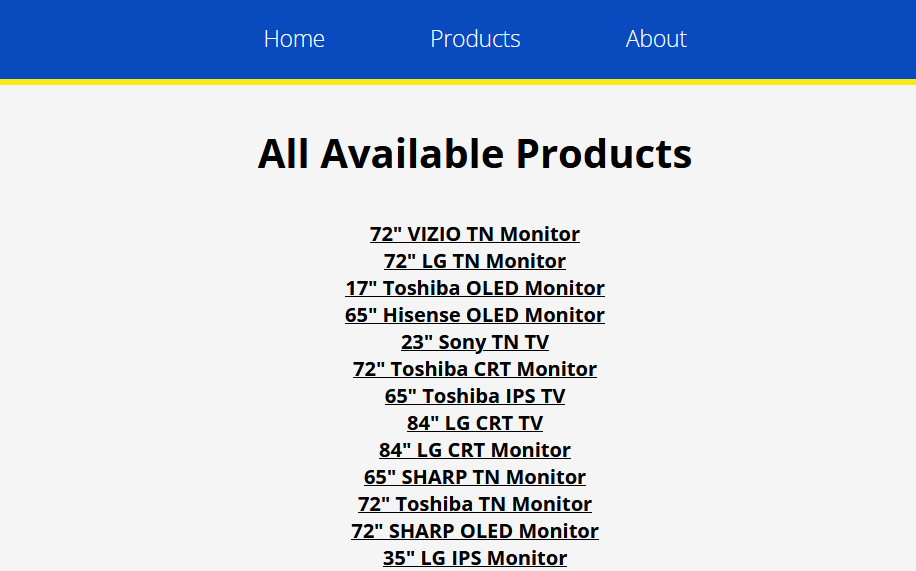
\includegraphics[width=0.48\textwidth]{Figures/allproducts.png} % Include the figure
	\caption{Picture of the product page.}
\end{figure}

\subsection{by UUID}\label{uuid}
The front-end functionality of this web page uses two key elements. An input element and a submit button. The input element is a type search, which enables the user to input anything they desire. In this case, the input is looking for the UUID of the user's desired product. The button is of type submit and is responsible for sending the user's input to the back-end. In order for a match to be found, the user must type in the exact UUID in order for results to show, else, the database will return empty. \par
The UUID is simply passed back to the view, this time through a POST call containing the desired UUID. Using python in this page's view function, the application performs a filter() query for any products with a matching UUID then sends the matching products to the HTML template to generate the new page.

\begin{figure}[H] % [H] forces the figure to be placed exactly where it appears in the text
	\centering % Horizontally center the figure
	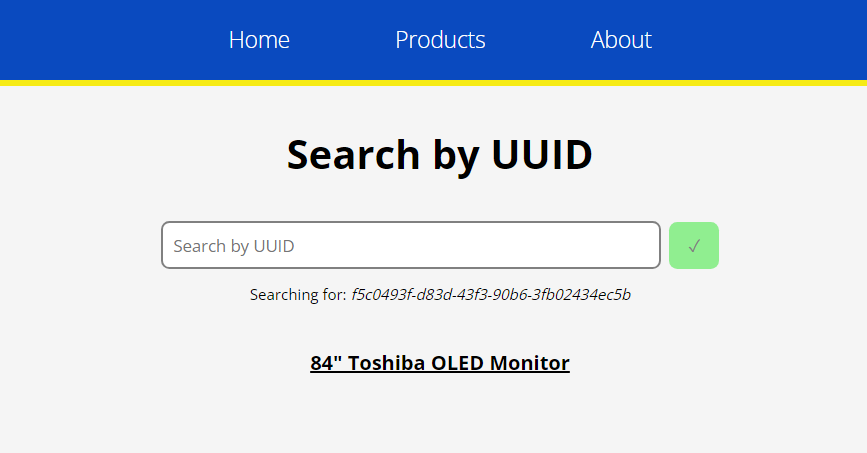
\includegraphics[width=0.48\textwidth]{Figures/exactmatch.png} % Include the figure
	\caption{Picture of the UUID page.}
\end{figure}

\pagebreak
\subsection{Best Match}\label{best}
The front-end functionality of this web page is quite dense and rigidly organized. It can be characterized into eight sections or input fields.
Four of which are drop-down menus and the rest are input text boxes. Each section is labeled by the feature or characteristic of the product that's to be searched. Furthermore, before each section label are small input boxes with a range of one to eight responsible for dictating the priority of each feature. There is a submit button to send this data to the back-end. \par
Due to the unique nature of this feature, the back-end functionality is quite complicated. Once receiving the data provided by the search submission, significant work is done parsing, reorganizing, and restructuring the data to be more workable. Once the different feature queries are all separated and linked up with their corresponding priority values, a chain of database queries are performed. First, the highest priority query is performed and stored. Then, the query of the next priority is performed, then a check is performed to determine if any results were found. If not, the search is cut short and the last set of results are returned. Otherwise, it continues down the priority list until all queries are performed or an empty query is returned. It then prints out the matching products, similarly to the previous page.

\begin{figure}[H] % [H] forces the figure to be placed exactly where it appears in the text
	\centering % Horizontally center the figure
	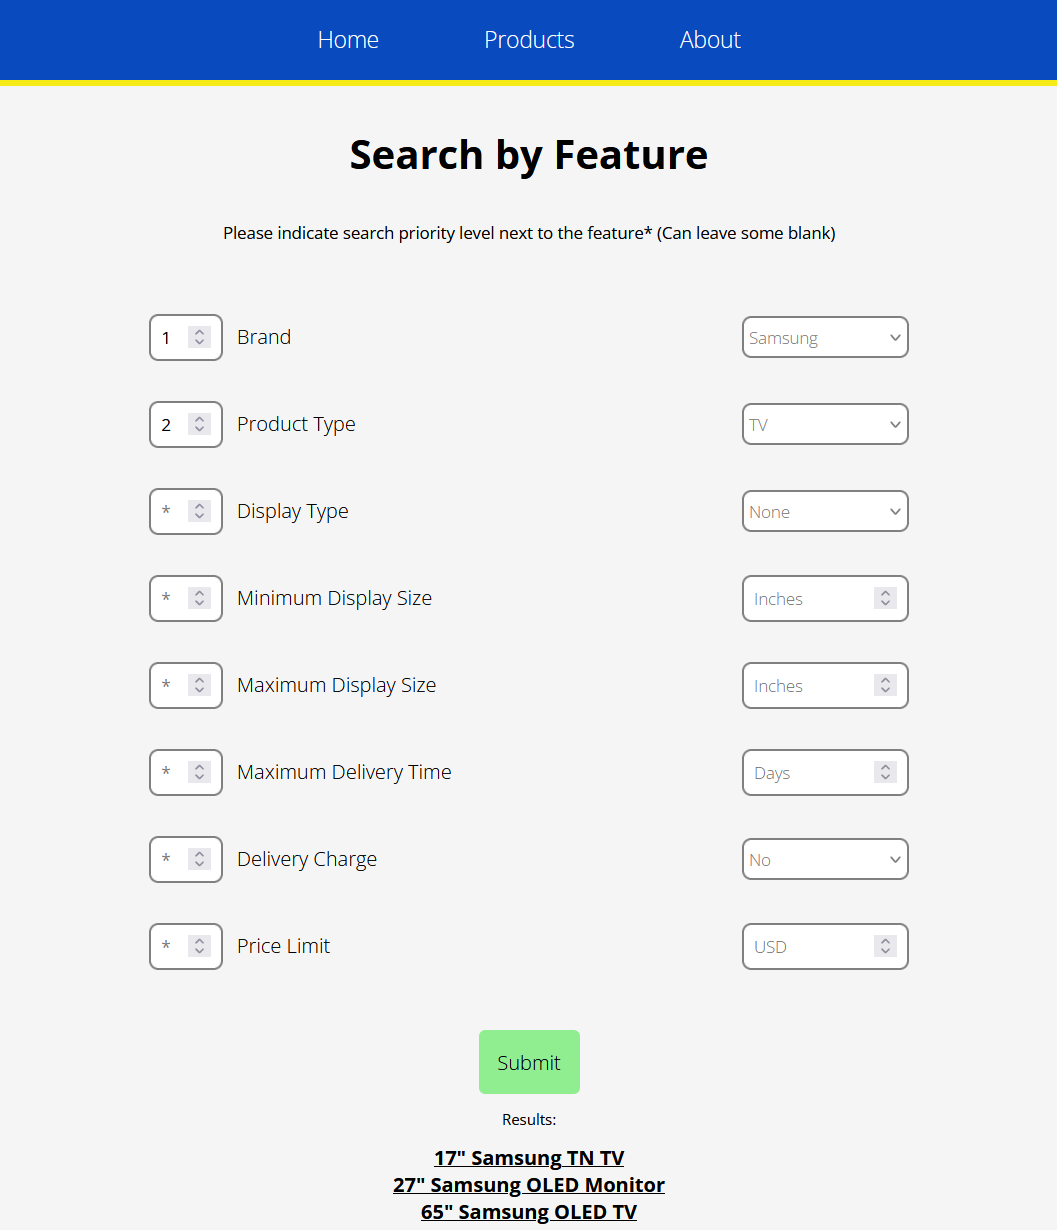
\includegraphics[width=0.47\textwidth]{Figures/bestmatch.png} % Include the figure
	\caption{Picture of the best match page.}
\end{figure}

\pagebreak
\subsection{by Feature}\label{feature}
The front-end functionality of this web page is very much similar to that of the 'Best Match' page but the back-end functionality is quite different. There are the eight sections alongside their feature labels and accompanying input types. There is no priority input in this criterion for the features. There is a submit button to send this data to the back-end. \par
On the back-end this feature works very similarly to the Best Match search. Depending on the criteria selected, database queries are chained one after the other, shrinking the pool of results for every criteria. No special data processing is needed, however, as there is no dynamic priority tied to each search criteria, and the queries can simply be chained one after another with no regard for order.

\begin{figure}[H] % [H] forces the figure to be placed exactly where it appears in the text
	\centering % Horizontally center the figure
	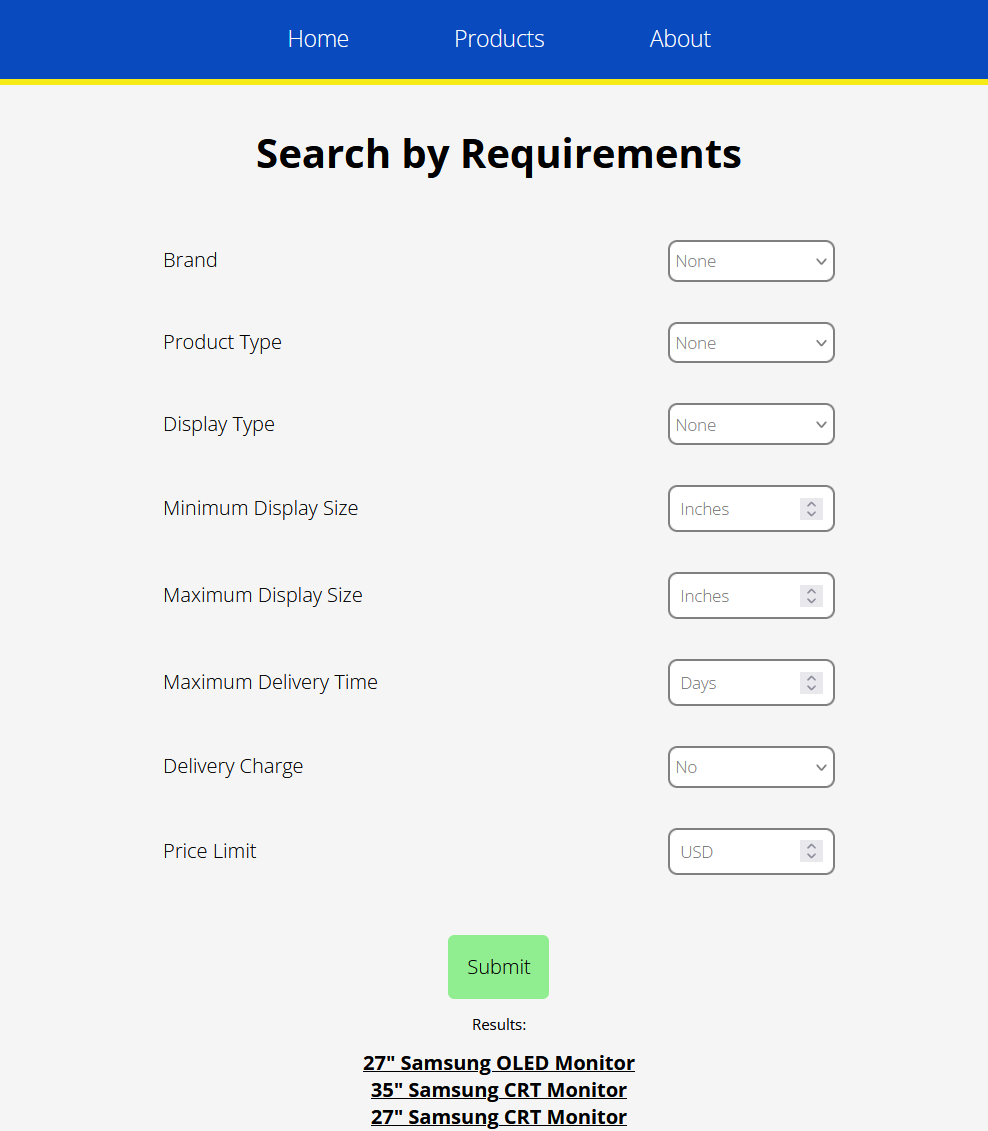
\includegraphics[width=0.47\textwidth]{Figures/requirements.png} % Include the figure
	\caption{Picture of the feature page.}
\end{figure}

\pagebreak
\section{Conclusion and Future Improvements}
In conclusion, we both found this project to be quite challenging but meaningful. This was our first real exposure to front-end and back-end development. To be thrown into such a project and to learn all these different things certainly made us more acknowledged to the functionality behind the Internet and data basing. We found that making a mock online store was an effective strategy and goal for our level of expertise. We are satisfied with what we managed to develop, though we would make some changes were we to do it again. First off, although we enjoyed learning Django, we would consider a web framework utilizing JavaScript, particularly Vue.js because we find that it might suit us better. Furthermore, we would likely flesh out and redo our relational models of our data base to add even more normalization and attributes. In terms of the website design, we would most certainly try to improve on the look and make it more modernized. In short, future improvements can be made, so far as to changing the framework, but what we managed to create looks clean and functions accordingly.

\bibliographystyle{ACM-Reference-Format}
\bibliography{sample-base}

\end{document}